\documentclass[10pt,letterpaper]{article}
\usepackage[top=0.85in,left=2.75in,footskip=0.75in]{geometry}

% amsmath and amssymb packages, useful for mathematical formulas and symbols
\usepackage{amsmath,amssymb}

% Use adjustwidth environment to exceed column width (see example table in text)
\usepackage{changepage}

% Use Unicode characters when possible
\usepackage[utf8x]{inputenc}

% textcomp package and marvosym package for additional characters
\usepackage{textcomp,marvosym}

% cite package, to clean up citations in the main text. Do not remove.
\usepackage{cite}

% Use nameref to cite supporting information files (see Supporting Information section for more info)
\usepackage{nameref,hyperref}

% line numbers
\usepackage[right]{lineno}

% ligatures disabled
\usepackage{microtype}
\DisableLigatures[f]{encoding = *, family = * }

% color can be used to apply background shading to table cells only
\usepackage[table]{xcolor}

% array package and thick rules for tables
\usepackage{array}

% create "+" rule type for thick vertical lines
\newcolumntype{+}{!{\vrule width 2pt}}

% create \thickcline for thick horizontal lines of variable length
\newlength\savedwidth
\newcommand\thickcline[1]{%
  \noalign{\global\savedwidth\arrayrulewidth\global\arrayrulewidth 2pt}%
  \cline{#1}%
  \noalign{\vskip\arrayrulewidth}%
  \noalign{\global\arrayrulewidth\savedwidth}%
}

% \thickhline command for thick horizontal lines that span the table
\newcommand\thickhline{\noalign{\global\savedwidth\arrayrulewidth\global\arrayrulewidth 2pt}%
\hline
\noalign{\global\arrayrulewidth\savedwidth}}


% Remove comment for double spacing
%\usepackage{setspace} 
%\doublespacing

% Text layout
\raggedright
\setlength{\parindent}{0.5cm}
\textwidth 5.25in 
\textheight 8.75in

% Bold the 'Figure #' in the caption and separate it from the title/caption with a period
% Captions will be left justified
\usepackage[aboveskip=1pt,labelfont=bf,labelsep=period,justification=raggedright,singlelinecheck=off]{caption}
\renewcommand{\figurename}{Fig}

% Use the PLoS provided BiBTeX style
\bibliographystyle{plos2015}

% Remove brackets from numbering in List of References
\makeatletter
\renewcommand{\@biblabel}[1]{\quad#1.}
\makeatother



% Header and Footer with logo
\usepackage{lastpage,fancyhdr,graphicx}
\usepackage{epstopdf}
%\pagestyle{myheadings}
\pagestyle{fancy}
\fancyhf{}
%\setlength{\headheight}{27.023pt}
%\lhead{\includegraphics[width=2.0in]{PLOS-submission.eps}}
\rfoot{\thepage/\pageref{LastPage}}
\renewcommand{\headrulewidth}{0pt}
\renewcommand{\footrule}{\hrule height 2pt \vspace{2mm}}
\fancyheadoffset[L]{2.25in}
\fancyfootoffset[L]{2.25in}
\lfoot{\today}

%% Include all macros below

\newcommand{\lorem}{{\bf LOREM}}
\newcommand{\ipsum}{{\bf IPSUM}}

%% END MACROS SECTION


\begin{document}
\vspace*{0.2in}

% Title must be 250 characters or less.
\begin{flushleft}
{\Large
\textbf\newline{From treadmill to trails: predicting performance of runners} 
}
\newline
% Insert author names, affiliations and corresponding author email (do not include titles, positions, or degrees).
\\
B.~Crowell\textsuperscript{1}
\\
\bigskip
\textbf{1} Natural Science Division, Fullerton College, Fullerton, CA, USA\\
\bigskip

\end{flushleft}

\linenumbers

\section*{Abstract}

Previous laboratory studies have measured the energetic costs to humans of running at
uphill and downhill slopes on a treadmill. This work investigates the extension
of those results to the prediction of relative performance of athletes running
on flat, hilly, or very mountainous outdoor courses.
Publicly available race results in the Los Angeles area provided a set of
109,000 times, with 2200 runners participating in more than one race, so that
their times could be compared under different conditions.
I compare with the results of
a traditional model in which the only parameters considered are total distance
and elevation gain. Both the treadmill-based model and the gain-based model
have some shortcomings, leading to the creation of a hybrid model that combines
the best features of each.

% Use "Eq" instead of "Equation" for equation citations.
% For figure citations, please use "Fig" instead of "Figure".

\section*{Author summary}
Running a race on a road allows absolute measures of performance. Trail running, however, has traditionally
been thought of as a sport in which the only valid comparison is between
different runners competing on the same course on the same day. Even the
exact measurement of distance is considered to be unimportant, since courses
and conditions vary so much. 

An extreme example is the relatively new genre
of ``vertical'' races, in which runners race up a mountain.
In a typical example, the competitors cover a horizontal distance of 5 km,
while climbing about 1000 m. The winner in one such race had a time
almost triple that expected for a state-champion high school runner in
a 5k road race. Clearly no comparison can be made here without taking into account
the amount of climbing.

In noncompetitive contexts, many runners venture onto mountain trails,
lightly dressed and with little equipment, so that it becomes important to be able
to anticipate whether they will have the endurance needed to be able to safely complete a planned route.
Again, this is impossible without some model of the effect of hill climbing.

% high school 3 mi: Joshua Schuld, PCL Dual Meets, 2020, 14:16, https://www.athletic.net/CrossCountry/Division/List.aspx?DivID=54890

% Broken Arrow Vertical Kilometer, the competitors cover a horizontal distance of 5.0 km
% while climbing a total of about 900 m. The winner in 2019 had a time of 42:46,
% almost triple the time that would be expected for a state-champion high school runner in
% a 5k road race.

\section{Introduction}

This paper presents a method for predicting relative performance on trail runs --- ``relative''
meaning that we can predict the time for course A divided by the time for course B.

Traditionally, runners and hikers have described a trail using two numbers, the horizontal distance and the total elevation gain.
For example, if the route is an out-and-back voyage consisting of steady climbing to a peak and
a return, then the total elevation gain is simply the elevation of the peak minus the elevation of
the trailhead. If the elevation profile of the trip consists of multiple clearly defined ascents and descents,
then one adds up the ascents. Although this two-parameter description of the route is
easy to derive from a paper topographic map, knowledge of the two numbers is not sufficient
to make a very useful estimate of the total energy expenditure.

It has been known for a long
time among the officials who measure road races that the effect
of elevation change has a nonlinear dependence on the grade. The following argument 
was advocated by R.~Baumel.\cite{baumel}
Consider a closed course whose elevation
profile is described by some function $y(x)$. The derivative $y'$ is the trail's slope $i$.
The total energy expenditure is an integrated effect of the slope, of the form $\int_0^L C(i)dx$,
where $C$ is a function that describes the energetic cost of running up or down a hill.
We will see that $C$ has been measured in laboratory experiments, but for the moment we assume
only that $C$ is a smooth function, so that for small slopes it can be well approximated by the first few terms
of its Taylor series, $C(i)\approx c_0+c_1 i+c_2 i^2$. Then for any closed loop over a distance $L$,
the contribution from the $c_1$ term vanishes, and the energy cost is $c_0 L+c_2 \int_0^L i^2 dx$.
The dependence on the slope is therefore quadratic rather than linear. For example, if we were to exaggerate the
elevation profile by a factor of 2, $y\rightarrow 2y$, then the size of the $c_2$ term would go up by
a factor of \emph{four}, not two (in the low-slope limit, on a closed course).

\begin{figure}[h]
\includegraphics[width=8cm]{figs/minetti/minetti.pdf}
\centering
\caption{The cost of running as a function of slope. Solid line: the function $C_t$, fit to Minetti's treadmill data, Eq \ref{eq:minetti-fit}. Dashed line:
the function $C_g$, Eq \ref{eq:gain-only}, with $c_0$ chosen to agree with Minetti's $C(0)$ and $c_g=6.0$.}
\label{fig:minetti}
\end{figure}

From conversations with runners and hikers, I have found that the result of Baumel's argument almost
always elicits total disbelief, especially when presented as a numerical example showing the extreme smallness
of the slope effect when the slope is small. One of the goals of this paper is to test this empirically.
As an alternative hypothesis, it is commonly believed that one can get a good measure
of the relative energy cost by taking the horizontal distance and adding in a term proportional to the total elevation gain.
If the total gain is determined down to a fine enough scale (which with modern technology has become
more practical), then this hypothesis is equivalent to the assumption that the cost of running is
given by a function of the form
\begin{equation}\label{eq:gain-only}
   C_g(i) = 
  \begin{cases}
     c_0, & i\le0 \\
     c_0(1+c_g i), & i\ge 0,
  \end{cases}
\end{equation}
whose graph is shaped like a hockey stick (dashed line in Fig \ref{fig:minetti}).
Popularly proposed rules are that 100 m of elevation gain is equivalent to either 400 m or 800 m of horizontal distance,
so that $c_g$ is said to be approximately in the range from 4 to 8. There is nothing mathematically impossible
about this hypothesis. A function $C(i)$ of this form evades Baumel's argument because its hockey-stick shape
is not smooth at $i=0$, and therefore cannot be approximated by its Taylor series.

In a more sophisticated approach, Minetti \emph{et al.}\cite{minetti} have used oxygen
consumption to measure the energy expenditure of runners on a treadmill at slope $i$, for both
running and walking.
The results are expressed as $C=(1/m)d E/d s$, where $m$ is the person's body mass,
$E$ is the energy expended, and $d s$ is the increment of three-dimensional distance, which
usually differs negligibly from the increment of horizontal distance $d \ell$.
$C$ has units of $\textup{J}/\textup{kg}\cdot\textup{m}$. The correctness of the factor
of $1/m$ has empirical support.\cite{shaw}

Efficiency varies by $\sim25\%$ even among elite athletes,\cite{minetti}\cite{lucia}
and differences are also to be expected between elite and recreational athletes. This is one
of the reasons why this study presents a comparative technique, rather than an absolute method for
determining a particular runner's actual energy expenditure in units of kilocalories.

The function $C(i)$, shown as the solid line in Fig \ref{fig:minetti}, resembles a hyperbola, with a
minimum occurring at $i\approx -0.1$ to $-0.2$. 
The asymptotes
at large positive and negative values of $i$ are interpreted in \cite{minetti} as being determined by the
efficiency of eccentric and concentric muscle contraction. For the purposes of this work, a new analytic
approximation to the curve found by ref.~\cite{minetti} is used (Appendix 1), and is referred to as
$C_t$, where ``t'' stands for ``treadmill.''

Nearly all real-world walking and running is
done at $-0.2 \lesssim i \lesssim 0.2$, where the graph of $C(i)$ is nearly parabolic.

\section{Methods}

\subsection{Analysis of publicly available race data}

To test these models, I use publicly available race results from the Los Angeles area.
This area has a large population and tall mountains. The large population makes it possible
to pick out a significant number of runners who have competed in several different races.
If the ratio of the runner's time on courses 1 and 2 is $t_2/t_1$, then we take this
as a measure of the ratio $E_2/E_1$ of the energy expenditure, which can be compared with
the model. It was possible to find courses with a variety of elevation profiles, allowing
a test of the dependence of the predictions on the amount of hill climbing.

\begin{table}[h]\label{table:courses}
\caption{Courses used in this study. Notes: 1.~Times up to 2:30 were used. 
2.~Times up to 1:11 were used for course S. A map of course S was not available, so a flat elevation profile was
assumed.
}
\begin{tabular}{lp{60mm}rrrl}
                 &       & dist.  & gain &  &  years \\
                 &       & (km)      &  (km) & CF & (20xx) \\
W & Mount Wilson Trail Race         & 12.7 & 0.70 & 20\%        & 18-19\\
B & Mount Baldy Run to the Top      & 10.3 & 1.21 & 47\%        & 17-18\\
V & Broken Arrow Vertical Kilometer & 5.0  & 0.85 & 58\%        & 19 \\
P & Pasadena Half Marathon\textsuperscript{1}
                                    & 21.1 & 0.17 & 1\%         & 17-20 \\
C & Agoura Hills Chesebro Half Marathon\textsuperscript{1}
                                    & 21.1 & 0.34 & 5\%     & 19 \\
H & Into the Wild OC Half Marathon\textsuperscript{1}
                                    & 21.1 & 0.57 & 8\% & 17-18\\
I & Irvine Half Marathon\textsuperscript{1}
                                    & 21.1 & 0.09 & 0.2\% & 19-20\\
G & Griffith Park 30k
                                    & 28.5 & 1.07 & 11\%        & 18-19 \\
X & Revel Big Bear Half Marathon\textsuperscript{1}
                                    & 21.1 & 0    & -27\% & 18-19 \\
S & Santa Monica 10k Classic\textsuperscript{2}        & 10 & & & 19\\
\end{tabular}
\label{table:courses}
\end{table}

Table \ref{table:courses} lists the races used as sources of data.
One-letter mnemonics are defined so that courses can be referred to succinctly in the text.
Because a runner's performance can change over time due to training and aging,
the time period of the study was restricted as much as possible to January 2017 through March 2020
(before the COVID epidemic ended races other than virtual ones in California).
Distance and elevation data were analyzed as described in Appendix 3.

Runners' names and times were obtained by web-scraping public race results,
and runners were assumed to be the same person if their first and last names matched.
When a runner ran the same race more than once, their best time was used.
To avoid biases in comparisons of times in different races, it is necessary here to define
an upper limit on the times that will be used from a given race, and to do so in some
consistent and unbiased way. Some such limit is in any case
defined by race organizers, but is different for different races and usually quite long,
often about 4-5 hours for a half-marathon. Competitors who clock the longer times are generally
either walking the entire race or alternating between walking and jogging, and especially in
more casual races may be pushing a stroller, running alongside their tween-age child, or staying
in a costumed group for fun and emotional support. Because the physiological data and models
used in this work are not applicable to walking, I impose a somewhat arbitrary time limit of 2.5 hours
on half-marathon times. These limits, as well as others, where imposed,
are described in the notes in Table \ref{table:courses}. For course S, the time limit was derived by
scaling down the half-marathon time limit in proportion to the distance.
The other courses in this study are of a qualitatively different character, so for them I simply
used the race organizers' cut-off. The resulting bias is an inherent limitation of this work.

Exertion depends most strongly on distance, and the goal of this work is to tease out effects
from other factors, which are often weaker. For this reason, distance is a confounding variable
in this study and has been controlled for as much as possible by using races at a consistent
distance, the half marathon (21.1 km), or distances that, taking extreme climbing into account,
result in similar times. These are the distances at which the largest sample sizes are available for
mountain trail races. Section \ref{sec:endurance} describes how the remaining inevitable
variations in distance have been taken into account, as much as possible.

In table \ref{table:courses}, two measures of hilliness are given. The total elevation gain
is the only parameter needed in order to calculate an energy expenditure using the function
$C_g$. The next column gives a statistic I will refer to as the climb factor, CF, which is
defined as the fraction of the runner's total energy expenditure that is devoted to climbing.
That is, if $E$ is the actual energy required for the course, and $E_0$ the energy that
would have been required if the race had been perfectly flat, then 
\begin{equation}
  CF=\frac{E-E_0}{E}.
\end{equation}
Inverting this equation gives $E=E_0/(1-CF)$, so that if the horizontal distance is
known, a measure of effort can be found by dividing the distance by $1-CF$.

To define quantitative tests of the models, consider a comparison
of courses 1 and 2. The observed data are the runner's times $t_1$ and $t_2$, and
the model predicts the ratio of the energy consumption $E_1/E_2$. Define
\begin{equation}\label{eq:define-e}
  \mathcal{E} = 100 \ln\left(\frac{t_1}{t_2}\cdot\frac{E_2}{E_1}\right).
\end{equation}
For small errors, $\mathcal{E}$ is approximately the relative error in the prediction, expressed
as a percentage. The use of the logarithm transforms multiplicative sources of
error into additive quantities.

We pick a feature of the model that is to be tested. For example, we would like to see
whether the model does a good job of predicting the relative times for flat races
compared to steep uphill-only races (Fig \ref{fig:test-hockey}, c). For this example, we make a list of courses
that are relatively flat (P, C, H, and I), and a list of some that are steep uphill-only
courses (B and V). We then find every case where the same runner did a run $j$ from the first
list and a run $k$ from the second, and compute the error $\mathcal{E}_{jk}$, which will be
positive if the runner's time in the uphill race $k$ is overpredicted by the model relative
to their time in the flat race $j$.

\subsection{Model of endurance}\label{sec:endurance}

Animals run more slowly at long distances, and mathematical modeling of this fact dates back
about a century.\cite{hill}  Recent workers have described methods for fitting parameters
to the data for individual runners,\cite{rapoport}\cite{emig} which for example allows
a first-time marathon runner to estimate an appropriate pace. In the present work, there are
not enough data available to allow this kind of individualized description of the runners.
For this reason, I have concentrated on data from a narrow range of middle distances,
with the total energy expenditure being close to that of a flat half-marathon road race.
But the endurance required for these races does vary, and this makes it desirable to have
some rough method of compensating for the variation in pace with distance. Here I describe
a very simple model that has the following characteristics that make it suitable for this
study: (1) its two parameters are universal rather than fits to the characteristics of an individual;
(2) its dependence on the parameters is purely multiplicative, i.e., varying the parameters only
rescales the axes on a graph of speed versus distance.
The model is essentially a simplification of the one constructed by Rapoport,\cite{rapoport} with modifications
to suit these purposes.

First we compute an equivalent distance $d$, which is the distance of flat running that would
require the same energy expenditure as the actual run. If the runner's time is $t$, then
$v=d/t$ has dimensions of speed, but is in fact a measure of energy per unit time, or power.
We then have
\begin{equation}\label{eq:fuel-model-1}
  Pt=d/\epsilon,
\end{equation}
where $P$ is the power and $\epsilon$ is a measure of the runner's efficiency. For example,
a recreational runner with a slight roll of belly fat will have a lower value of $\epsilon$ because of
the increased energetic cost of transporting the additional body weight. Although it would seem that
we are now introducing an individualized parameter $\epsilon$, the model is designed so that at the
end of the calculation, cancellations occur that allow $\kappa$ to be predicted on a universal basis.

The power $P$ depends on aerobic fitness and on the proportions of fat and carbohydrates being
burned in aerobic metabolism. Fat burning is slower than carbohydrate burning by a factor $\beta\approx 0.4$.\cite{rapoport}
If we let $f$ be the fraction of energy production from carbohydrates, then
\begin{equation}\label{eq:fuel-model-2}
  P = A[f+\beta(1-f)],
\end{equation}
where the proportionality constant $A$ is another per-individual parameter that it will be
possible to normalize away later. This expression's linearity in $f$ is an approximation to
results from real-world data that provide evidence for slightly nonlinear behavior.\cite{rapoport}

The runner's supply of carbohydrates $c$ is limited by the amount of glycogen that can be stored
in the liver and the leg muscles. If $f$ is chosen optimally, then there will be some distance
$d_c=c\epsilon$ that can be run with pure carbohydrate fuel, while longer distances will require $f<1$.
Thus,
\begin{equation}\label{eq:fuel-model-3}
  f = \begin{cases}
    1, & d\le d_c \\
    c/At, & d\ge d_c.
\end{cases}
\end{equation}
Under these assumptions, the runner's speed will be the same in races at all distances less than $d_c$,
which is unrealistic. We will first work out the consequences of Eq \ref{eq:fuel-model-1}-\ref{eq:fuel-model-3}
and the introduce a simple elaboration that more realistically reproduces the effects of fatigue.

Solving Eq \ref{eq:fuel-model-1}-\ref{eq:fuel-model-3} and expressing $\kappa$ as a correction factor
relative to the short-distance maximum speed $v_m=A\epsilon$, we find
\begin{equation}\label{eq:kappa-simple}
  \kappa_0 = \begin{cases}
    1, & d\le d_c \\
    \frac{\beta}{1-(1-\beta)d_c/d}, & d\ge d_c.
  \end{cases}
\end{equation}
This depends on the universal parameter $\beta\approx0.4$ and also on the critical distance $d_c$.
The latter is a measure of endurance and does depend on individual factors such as
body composition and training, as well as on strategies such as carbohydrate loading.
However, for the sample of recreational athletes studied here, I hypothesize that one can fix a universal value of $d_c$ lying somewhere
around the half-marathon distance, and find a reasonable description of
real-world data.

\begin{figure}[h]
\includegraphics[width=8cm]{figs/my-times/my-times.pdf}
\centering
\caption{Relative speed versus equivalent distance $d$. All speeds are normalized relative to the speed at half-marathon distance.
The black curve is the function defined by Eq \ref{eq:kappa}, with $d_c$ set to a half-marathon distance.
The red curve is a 
fit to world-record times.\cite{cameron} 
The green and red violin plots show the distribution of speeds in races S and G relative to the same runners
in half-marathon race P (sample sizes 1303 and 11, respectively).
The gray dots are the author's personal-record times from a variety of courses.
The equivalent distances were determined from the horizontal distances using the curvilinear
function $C_t(i)$ in Eq \ref{eq:minetti-fit}, which is based on treadmill data. }
\label{fig:my-times}
\end{figure}

It is not true in reality that runners can maintain the same pace at any of the distances below
$d_c$, for which glycogen suffices. As the distance increases from 5 km to the half-marathon
distace of 21 km, one observes a decrease in speed which, as originally observed by Hill,\cite{hill} appears
linear on a graph of speed versus the logarithm of distance. In the men's and women's world-record
times, this decrease is about 5\%. The graph then shows a knee, like the one described by Eq \ref{eq:kappa-simple}.
The more gradual decrease for distances before the knee is generically described as being due to fatigue, which is
a complicated and poorly understood phenomenon involving a variety of factors, many of which are mediated
by the central nervous system rather than by any change at the chemical or tissue level. As an \emph{ad hoc}
correction, we multiply the result of Eq \ref{eq:kappa-simple} by a factor
controlled by a small parameter $Q$:
\begin{equation}\label{eq:kappa}
  \kappa = \left(\frac{1+(1-3Q)d/d_c}{1+d/d_c}\right) \kappa_0.
\end{equation}
The factor of 3 is introuced so that $Q$ is approximately equal to the reduction in speed between a 5k and a half-marathon,
and we set $Q=0.05$.

Empirically, for the mostly recreational runners studied here, a reasonable description of the data is achieved when
$d_c$ is set to the half-marathon distance, which is the value adopted in this work.
Fig \ref{fig:my-times} shows that
setting $d_c$ to half-marathon distance gives a good fit to some real-world data.

Although the fit in Fig \ref{fig:my-times} is rather good,
much higher values of $d_c$ might be more appropriate for higher-level endurance runners.
For example, Eliud Kipchoge's personal-record
speed is only 8\% lower in the marathon than in the 1500 m. This can only be reproduced in this model if $d_c$
is roughly marathon distance for him.
For high-level running competitions, Gardner and Purdy give a
method of comparing with a standard performance curve, based on a compilation of world
records.\cite{gardner} 
The red curve in Fig \ref{fig:my-times} is an approximation to the locus of world-record times (Appendix 2).

Although fitting parameters to individual runners' characteristics is not the main purpose of this work, doing
so is very easy with the model \ref{eq:kappa}, due to its purely multiplicative structure.
When data are viewed in the format used in Fig \ref{fig:my-times}, as a log-log plot of speed versus distance,
the standard curve $\kappa(d)$ is simply slid around horizontally and vertically to match the data, which
has the effect of determining the runner's $v_m$ and $d_c$.

\section{Results}\label{subsec:hills}

Fig \ref{fig:test-hockey} shows a comparison of the quality of the predictions of the functions
$C_g$ and $C_t$ as descriptions of the effects of going up and down hills.
The third model $C_r$ is a hybrid of these, introduced in section \ref{sec:hybrid}.
All predictions were corrected for distance as described in section \ref{sec:endurance}.
Each of the four sub-figures a through d has been constructed so as to test a particular
feature of these models. We discuss each in turn.

\begin{figure}[h]
\includegraphics[width=132mm]{figs/test-hockey/test-hockey.pdf}
\centering
\caption{Tests of the predictions of the functions $C_t$ derived from treadmill data (open circles),
$C_g$ based on eleveation gain (black circles), and the hybrid ``recreational'' model
$C_r$ (gray circles). Positive $\mathcal{E}$ means that the runner's
time in the first-listed race is greater in reality than in the model.
}
\label{fig:test-hockey}
\end{figure}

(a) Here we compare the extremely flat half-marathon I, having only 90 m of elevation gain,
to half-marathon P, which is slightly more hilly with 170 m of gain, or about twice as much.
According to the treadmill-based model $C_t$, the effects of climbing and descending
nearly cancel out, giving a negligible $CF<1\%$ for each run, as expected from Baumel's argument.
In the gain-based model $C_g$, however, the effect of the hills on course P is
6 times its elevation gain, which is equivalent to adding 1.0 km to its length. The effect for I would
be half as much, causing the model to predict a considerable difference in the times on
the two courses. In the figure we see that Baumel's approximation is a good one here. The median
error for $C_t$ (open circles) is only 1.7\%, while that for $C_g$ (filled circles) is +6.4\%,
the positive sign showing that the effect of the small hills is over-predicted.

Of the four tests a-d, this is the only one where the effect being probed is small enough to
require statistical analysis rather than simple visual inspection.
Such an analysis (Appendix 4)
show that systematic error in $C_g$ is significant ($p=3\times10^{-6}$), while any such evidence against
$C_t$ is statistically marginal.

(b) In this portion of Fig \ref{fig:test-hockey}, we compare times in a set of fairly flat half-marathons
(with CF values ranging from 0.2\% to 8\%) with course W, a trail race up and down half of Mount Wilson, $CF=20\%$.
Although the distance of W is much shorter, most runners' times are only slightly lower. We see that both
models greatly underpredict the runners' times in the mountain race. Most of the running in this race is
on slopes with $|i|\approx 0.10$ to 0.15. A likely interpretation is that on the uphills, $C_g$ is an
underestimate (see c, below), while on the downhills $C_t$ is an underestimate. The race is run on a trail that is
mostly a narrow single track, with steep hillsides on the climber's right. Safety is likely to inhibit
many runners from going downhill at anything like the pace that would be possible for the   elite mountain runners in ref.~\cite{minetti}
on a treadmill, and trail etiquette dictates that they yield the right of way when encountering
people who are still on their way up.

(c) This test compares runners' times on the same flattish half-marathons with their performances in
two races, B and V, in which runners go up a mountain and finish at the top. Of the sample size of $n=32$, only
one person was on course V, a ``vertical kilometer''-style race which was run in Northern California.
Although both models systematically underestimated the difficulty of the uphill races ($\mathcal{E}<0$),
the underestimate is far more severe for $C_g$ than for $C_t$. Course B consists almost
entirely of climbing on grades $0.05<i<0.25$, at which $C_g$ is less than $C_t$ and is apparently a
considerable underestimate. Additional factors leading to $\mathcal{E}<0$ in both cases
are certain to include the aerobic challenge of finishing the race at an elevation of over 3000 m,
as well as the difficult footing on the final section.

(d) Here we compare the same set of fairly flat half-marathons with a road half-marathon, course X,
which consists entirely
of running \emph{down} a mountain. The downhill race is run along with a marathon, which
the race's organizers advertise as being extremely fast and a good way to achieve a ``BQ'' or
qualifying time for the Boston Marathon. Surprisingly, most runners' times in the downhill
half-marathon were only about 10 minutes shorter than in the flat ones, and quite a few runners in
the sample actually took longer for the downhill race. We have already seen evidence in part
b above that the high physiological efficiencies observed in the lab for downhill running may
not translate proportionately into speed. In W, the issues may have been safety and courtesy,
which would not have been relevant in this race on a wide asphalt road. A more likely explanation
here is that for recreational runners who have not trained extensively on steep hills, a long downhill of this
length can be physically difficult due to the strong eccentric strain on the quadriceps, as well as
testing the tensor fascia latae.

\section{Discussion}

\subsection{Interpretation of results}

Fig \ref{fig:features} presents a graphical summary of the interpretation of these results.

\begin{figure}[h]
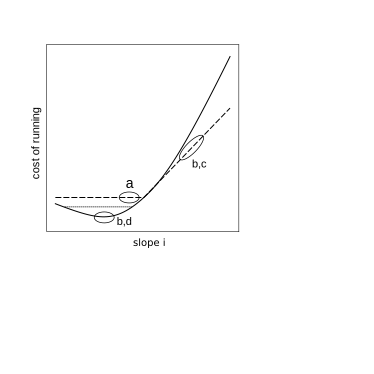
\includegraphics[width=73mm]{figs/features/features.pdf}
\centering
\caption{A graphical summary of the interpretation of the systematic errors in the models $C_t$ and $C_g$, observed
in parts a, b, c, and d of Fig \ref{fig:test-hockey}. Portions of the model that are
interpreted as being inaccurate are circled and labeled with the test that provides the
evidence for the inaccuracy. The interpretation is more conjectural for b, since both
models had similar errors, but hypothetically for different reasons.
The solid line is the treadmill-based function $C_t$ and the dashed one $C_g$.
The dotted line is a modified version $C_r$ of the treadmill function, defined in Eq \ref{eq:rec} and found
here empirically to be more appropriate for recreational runners in real-world trail conditions.}
\label{fig:features}
\end{figure}

The observations mainly support the model $C_t$, except that as
downhill grades get steeper and steeper, it appears that most
recreational runners in real-world conditions reach a point of
diminishing returns far earlier than is the case in treadmill studies.
The results for course X, which has an average $i\approx -0.05$,
suggest that this point of diminishing returns is reached at relatively
small negative slopes, perhaps $i\approx -0.03$.
The factors causing this effect probably have as much to do with safety and etiquette as
with physiology, so that they cannot be quantified in any
universal way. However, it would be irresponsible to provide runners,
especially recreational athletes, with scientific advice that would
give an unrealistically rosy picture of the difficulty of a run.

\subsection{Hybrid model}\label{sec:hybrid}

I have therefore investigated some possible modifications to the function
$C_t$. A modification that did not work well was to adjust the values of the parameters $p$ and $d$
given in Table \ref{table:minetti-params} so as to shift the minimum of
the function up and to the right. This was unsuccessful, because the smooth
analytic character of Eq \eqref{eq:minetti-fit} makes it impossible, by varying its parameters, to 
dramatically modify the function's behavior for $-0.06\lesssim i \lesssim -0.03$
while retaining its apparently correct behavior at $-0.03 \lesssim i \lesssim 0$.
A more successful ad hoc recipe was simply to introduce a cut-off in $C$, i.e.,
to define a ``recreational'' version of the function,
\begin{equation}\label{eq:rec}
  C_r =   \begin{cases}
     C_t(i), & C_t(i)>C_t(i_0) \\
     C_t(i_0), & \text{otherwise},
  \end{cases}
\end{equation}
where $i_0=-0.03$.
In other words, we simply chop the bottom off of the curve of $C_t$, at the dotted
line in Fig \ref{fig:features}.

The results of the hybrid model $C_r$ are shown as gray circles in Fig \ref{fig:test-hockey}
and are in general fairly good. The main remaining inaccuracy is the underprediction of the
effect of steep hills in test c. It would be tempting to modify the function $C$ to give it
an even more severe upward curve for $i\gtrsim 0.3$. This does not seem warranted by the present
data, since other factors may be at work, including altitude and rough footing.

\section{Conclusions}
This paper presents a model that can be used to predict the time of a runner on a
course, given their time on some other course. This model is a hybrid of two others that have been previously
proposed. Testing against a sample of times
clocked by mostly recreational athletes shows that
the model usually gives predict corrections
to within about 10-20\%, even when the route includes extreme climbing or descents.
It would be desirable for future work to refine this work by controlling better for factors such
as altitude, training, and the quality of footing on mountain trails.

\subsection*{Appendix 1. Analytic approximation to the treadmill function $C_t$}

It is convenient to describe the function $C(i)$ using a fit to the form
\begin{equation}\label{eq:minetti-fit}
  C_t(i) = a\left[(|i|^p+b)^{1/p}+\frac{i}{c}+d\right],
\end{equation}
where the subscript $t$ stands for treadmill.
Parameters fitted to the results of ref.~\cite{minetti} are given in Table \ref{table:minetti-params}.
The purpose of using this form, rather than the polynomial fit given by \cite{minetti}, is
to make the computations degrade gracefully in cases where the limitations of GPS tracks or data from digital elevation models
produce unrealistically steep slopes. In such cases, this expression approaches the physiologically
expected asymptotic behavior. Although the present work focuses only on running, parameters for walking
are presented as well. The results for running are empirically found to be nearly independent of speed,
whereas the ones for walking are not. For walking, ref.~\cite{minetti} measured the energy consumption
at the speed that was found to be most efficient for that
particular subject.

\begin{table}[h]
\caption{Parameters for Eq \eqref{eq:minetti-fit}. These parameters were found by constraining
Eq \ref{eq:minetti-fit} to agree with the polynomial fits in ref.~\cite{minetti} on the following
degrees of freedom: the function is minimized at the same $i$, and has the same value of $C$ there;
the functions agree at $i=0$. Furthermore, the slopes at $\pm\infty$ were constrained to have the asymptotic values
found in that work.}
\begin{tabular}{lll}
   & \emph{running} & \emph{walking} \\
$a$  & 26.07 $\textup{J}/\textup{kg}\cdot\textup{m}$ & 22.91 $\textup{J}/\textup{kg}\cdot\textup{m}$ \\
$b$  & 0.03104 & 0.02621 \\
$c$ & 1.381 & 1.315 \\
$d$ & -0.06547 & -0.08317 \\
$p$ & 2.181 & 2.209
\end{tabular}
\label{table:minetti-params}
\end{table}

\subsection*{Appendix 2. Analytic approximation to world-record speeds}

Cameron\cite{cameron} has given a
convenient closed-form approximation to world-record speeds of runners at various distances,
\begin{equation}\label{eq:cameron}
  v\propto 1-Ad+Bd^{-C}.
\end{equation}
This is shown as the red curve in figure \ref{fig:my-times}. The parameters are given in Table \ref{table:cameron-parameters}

\begin{table}[h]
\caption{Parameters for Eq \eqref{eq:cameron}, for $d$ in meters.}
\begin{tabular}{lll}
$A$ & $B$ & $C$ \\
$2.25\times10^{-6}$ & 61.9 & 0.790
\end{tabular}
\label{table:cameron-parameters}
\end{table}

% calc -e "A=13.49681; B=0.000030363; C=835.7114; D=0.7905; B/A; C/A"
%    2.24964269334754*10^-6
%    61.919179420915


\subsection*{Appendix 3: Analysis of elevation data}
Digital maps projected into a horizontal plane were obtained from the race organizers' web site
or in some cases by tracing roads and trails in a Google Maps application. Elevation data
were obtained from publicly available digital elevation models (SRTM1) having a horizontal
resolution of 30 meters. (Elevation data from handheld GPS/GNSS units are more difficult to
obtain from public sources, and are in any case of questionable reliability
for this purpose, since the uncertainty can be very large when all satellites are near the
horizon or when the terrain is rough, causing radio echoes from the walls of canyons.)

The use of these data is inherently subject to certain errors, which need to be minimized.
Trails and roads are intentionally constructed so as not to go up and down steep hills, but
the DEM may not accurately reflect this. The most common situation seems to be one in which
a trail or road takes a detour into a narrow gully in order to maintain a steady grade.
If the gully is narrower than the horizontal resolution of the DEM, then the DEM doesn't know about the the gully, and
the detour appears to be a steep excursion up and then back down the prevailing slope.

Empirically, I have found that sensitivity to these effects can be minimized if the elevation
profile of the run $y(x)$ is filtered by convolving it with a rectangular windowing function having width
$w=200$ meters. This tends to eliminate unrealistic glitches in the elevation data, and also seems to give
a fairly close reproduction of race organizers' estimates of total elevation gain. This choice of $w$ gives
sane results for routes in mountainous terrain, and is used throughout this work, even for flat courses
on city streets. For a course that is relatively flat and has many small, short hills, $w\approx60$ m gives
more accurate results, but I have used the larger value of $w$ throughout this work in an effort to maintain
consistency.

The mileage derived from a GPS track can vary quite a bit depending on the resolution of the GPS data.
Higher resolution increases the mileage, because small wiggles get counted in. This has a big effect on
the energy calculation, because the energy is mostly sensitive to mileage, not gain. For races
that were advertised as 5k or half-marathon races, I have therefore used the advertised distance,
as shown in Table \ref{table:courses},
in order to calculate the first-order estimate of the energy, but have used the elevation gain and
CF value derived from the actual GNSS data.

\subsection*{Appendix 4: Statistical analysis}

In section \ref{subsec:hills}, test (a) probes an effect small enough that visual inspection of the scatter plots is
not a satisfactory way of testing hypotheses. Specifically, we want to know whether
the apparent systematic error in the model $C_g$ is statistically consistent with zero.

We do not know a priori the underlying probaility distribution of the ratio of times or of its
logarithm $\mathcal{E}$. One might have expected based on
previous work\cite{godsey} that the times would be log-normal, in which case $\mathcal{E}$ would
be normally distributed. However, a Q-Q plot shows that this is not the case for the present
data-set, and in fact the distribution of $\mathcal{E}$ is asymmetric. The ratio of times,
however, has a symmetric and leptokurtic distribution. Its symmetry allows the use of the
one-sample Wilcoxon test.
For $C_g$ the null hypothesis is rejected with $p=4\times10^{-6}$, while
for $C_t$, $p=0.07$. Thus the defect in $C_g$ is significant, while any such evidence against
$C_t$ is statistically marginal.

% see significance.r

\section*{Acknowledgements}

The author thanks Wendy Yen for helpful conversations.

\section*{Data availability statement}

The compilation
of race times was derived from public sources and is itself publicly available at \url{https://github.com/bcrowell/trail}.
The code used to analyze the data is contained in that repository and in \url{https://github.com/bcrowell/kcals}.
All code is under a GPL license.
I have also used Zenodo to
assign a DOI to the data: 10.5281/zenodo.4661554.

% \bibliography{trail}

\begin{thebibliography}{1}

% PLOS wants Vancouver style.
% https://www.nlm.nih.gov/bsd/uniform_requirements.html
% Halpern SD, Ubel PA, Caplan AL. Solid-organ transplantation in HIV-infected patients. N Engl J Med. 2002 Jul 25;347(4):284-7.

\bibitem{baumel}
Baumel R. Hill effect to second order.
    Measurement News. 
    1989 Jan;33:36.
    %Available from: \url{http://www.runscore.com/coursemeasurement/MeasurementNews/033_89a.pdf}

\bibitem{minetti}
      Minetti AE, Moia C, Roi GS, Susta D, and Ferretti G.
      Energy cost of walking and running at extreme uphill and downhill slopes.
      J Applied Physiology.
      2002;93:1039.

\bibitem{shaw}
      Shaw AJ, Ingham SA, Folland JP.
      The valid measurement of running economy in runners 
       Med Sci Sports Exerc.
       2014 Oct;46(10):1968-73.

\bibitem{lucia}
      Lucia A, Olivan J, Bravo J, Gonzalez-Freire M, and Foster C.
      The key to top-level endurance running performance: a unique example.
      British Journal of Sports Medicine.
      2008;42(3):172.

, 42(3), 172–174. doi:10.1136/bjsm.2007.040725 

\bibitem{godsey} Godsey B. Comparing and forecasting performances in different events of athletics using a probabilistic model.
        Journal of Quantitative Analysis in Sports.
        2012 Jun;8(2):1. doi:10.1515/1559-0410.1434

\bibitem{hill} Hill AV. The physiological basis of athletic records. 
         Lancet. 1925;5:481-486.

\bibitem{rapoport} Rapoport BI. Metabolic factors limiting performance in marathon runners.
      PLoS Comput Biol.
       2010 Oct;6(10):e1000960.

\bibitem{emig} Emig T and Peltonen J. Human running performance from real-world big data.
        Nat Commun.
        2020 Oct 6;11:4936.
        doi:10.1038/s41467-020-18737-6

\bibitem{gardner} Gardner J and Purdy J. Computer generated track scoring tables.
        Medicine and science in sports. 2, 152–161.
        1970;2(3):152.

\bibitem{cameron}
     Cameron DF. Time-equivalence Model. 
     1998 Jun.
     Available from: \url{http://www.cs.uml.edu/~phoffman/cammod.html}




\end{thebibliography}


\end{document}

